%!TEX root = dolgozat.tex
%%%%%%%%%%%%%%%%%%%%%%%%%%%%%%%%%%%%%%%%%%%%%%%%%%%%%%%%%%%%%%%%%%%%%%%
\chapter{Preprocessing images}\label{ch:PREPROC}
%%%%%%%%%%%%%%%%%%%%%%%%%%%%%%%%%%%%%%%%%%%%%%%%%%%%%%%%%%%%%%%%%%%%%%%

In order to simplify the data the learning algorithm is going to work with, I preprocess the images based on their color. The neural network works with the gray value of the pixels. Because the images are taken in real life environment, they contain other objects (branches). They were taken in different light conditions; some of them ending up really obscure or blanch. 

\section{Color spaces}\label{sec:PREPROC:colorSpaces}

Color space is a method by which we can specify, create and visualize colors. A color is usually specified using three coordinates, or parameters. These parameters describe the position of the color within the color space. Different color spaces are better for different applications. 

\subsection{RGB color space}\label{sec:PREPROC:rgb}

RGB color space is an additive color system based on tri-chromatic theory. The tri-chromatic theory describes the way three separate %lights
, red, green and blue, can match any visible color. RGB is easy to implement but non-linear with visual perception. RGB is frequently used in most computer applications since no transformation is required to display information on the screen. RGB space may be visualized as a cube with the three axes corresponding to red, green and blue.

\begin{figure}[h]
\centering

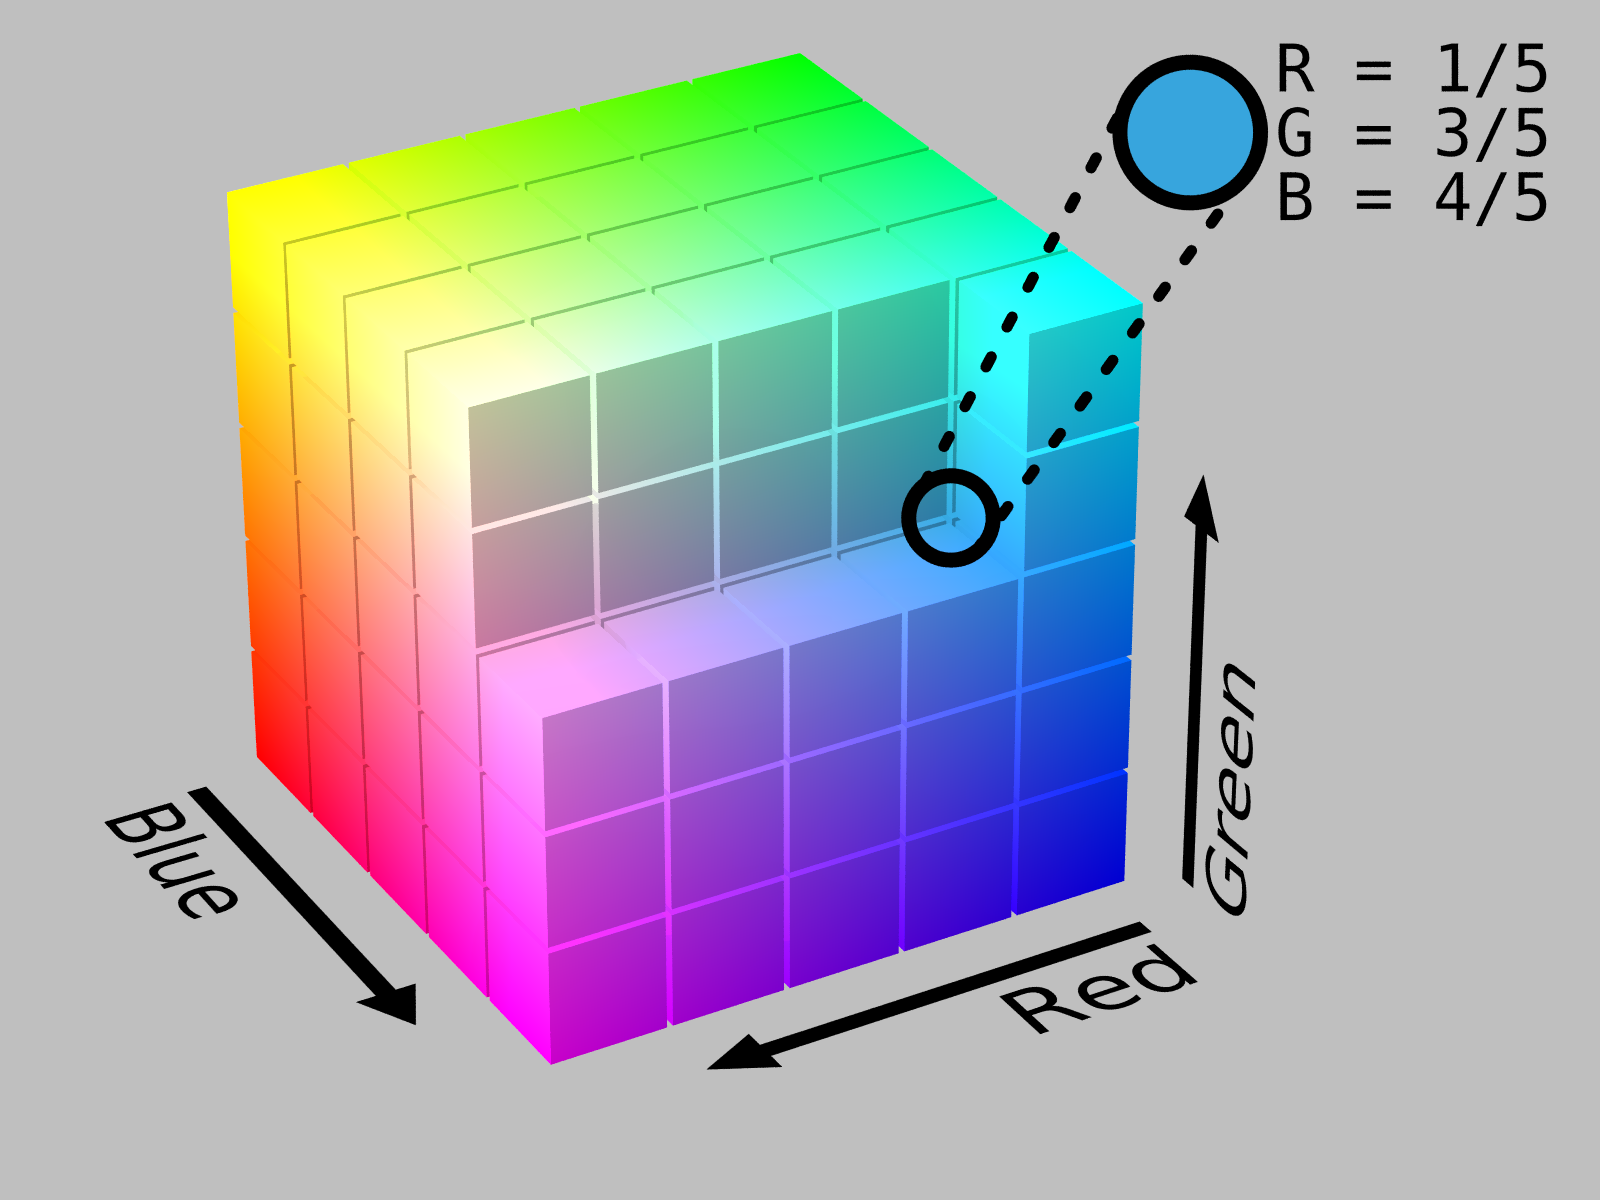
\includegraphics[scale=0.1]{RGBColorSpace}
\caption{RGB Color space}

\label{fig:RGBColorSpace}
\end{figure}

\subsection{HSV color space}\label{sec:PREPROC:hsv}

The HSV color space is one of the most common cylindrical-coordinate representations of points in an RGB color model. The hue is the human sensation according to which an area appears to be similar to one, or to proportions of two, of the perceived colors red, yellow, green and blue. The saturation is the colorfulness of an area relative to its brightness.  The value (brightness) is the human sensation by which an area exhibits more or less light. The color is then defined as a position on a circular plane around the value axes. Hue is the angle from a nominal point around the circle to the color while saturation is the radius from the central lightness axis to the color.

\begin{figure}[h]
\centering

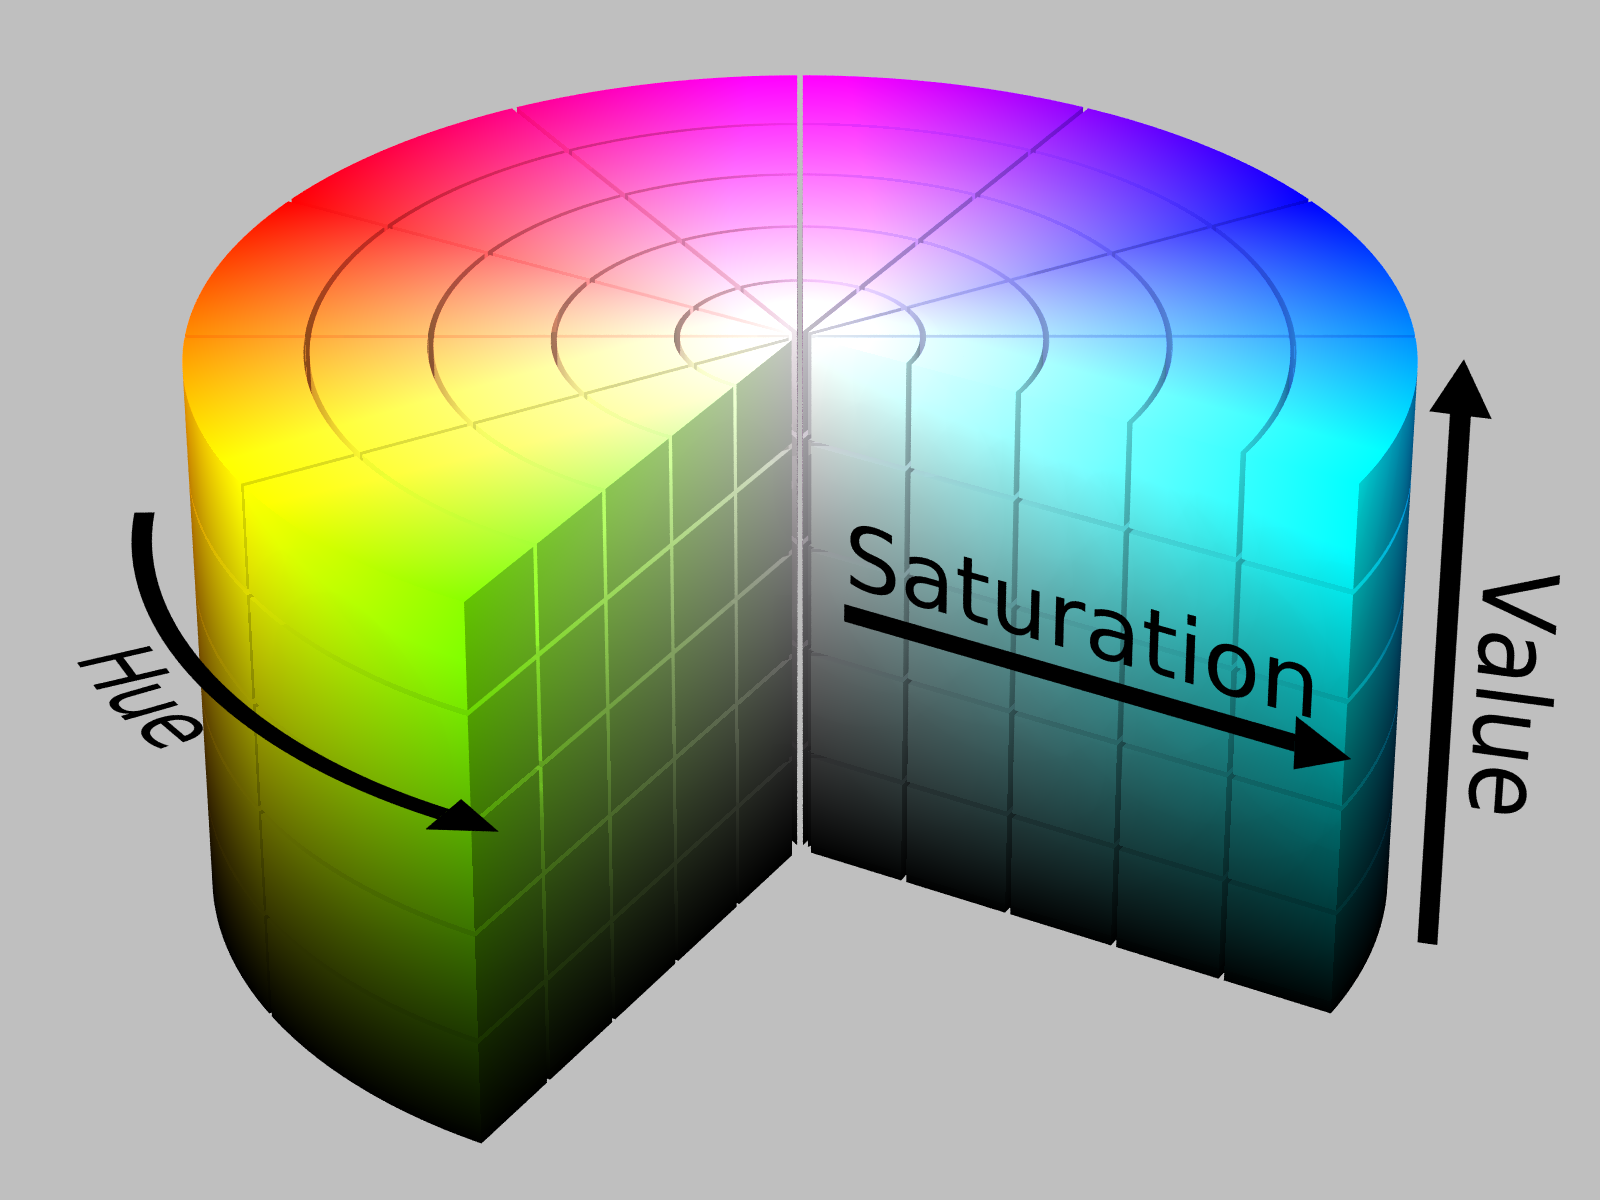
\includegraphics[scale=0.1]{HSVColorSpace}
\caption{HSV Color space}

\label{fig:HSVColorSpace}
\end{figure}

\section{Implementation}\label{sec:PREPROC:implement}



The traffic signs are meant to raise awareness therefore they use vivid colors, like red, yellow, blue, black, white. I create a new black and white image by filtering the colors of the original image. If the hue, saturation and value of a pixel satisfy a certain threshold, the pixel of the new image will be black otherwise white. I established these thresholds based on experiments and the \ref{fig:colorWheel} figure.

\begin{figure}[h]

\centering 
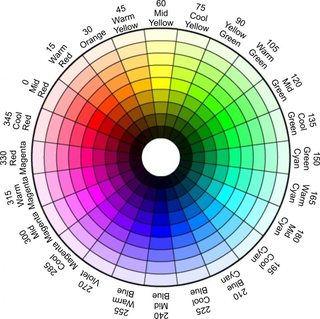
\includegraphics[scale=0.5]{ColorWheel}
\caption{Color wheel}
\label{fig:colorWheel} 

\end{figure}

%\begin{table}[H]
%\centering
%\begin{tabular}{ |p{3cm}||p{3cm}|p{3cm}|p{3cm}|  }
% \hline
% Country Name     or Area Name& ISO ALPHA 2 Code &ISO ALPHA 3 Code&ISO numeric Code\\
% \hline
% Afghanistan   & AF    &AFG&   004\\
% Aland Islands&   AX  & ALA   &248\\
% Albania &AL & ALB&  008\\
% Algeria    &DZ & DZA&  012\\
% American Samoa&   AS  & ASM&016\\
% Andorra& AD  & AND   &020\\
% Angola& AO  & AGO&024\\
% \hline
%\end{tabular}
%
%\caption{Table to test captions and labels}
%\label{table:1}
%\end{table}

